\documentclass[11pt,a4paper]{article}

% ============================================================
% PACKAGES
% ============================================================
\usepackage[utf8]{inputenc}
\usepackage[T1]{fontenc}
\usepackage[english]{babel}
\usepackage{amsmath, amssymb, amsthm}
\usepackage{geometry}
\geometry{margin=2.5cm}
\usepackage{graphicx}
\usepackage{xcolor}
\usepackage{listings}
\usepackage{hyperref}
\usepackage{booktabs}
\usepackage{array}
\usepackage{tikz}
\usetikzlibrary{arrows.meta, positioning, shapes, calc}
\usepackage{enumitem}

% ============================================================
% CONFIGURATION
% ============================================================
\hypersetup{
    colorlinks=true,
    linkcolor=blue,
    urlcolor=blue,
    citecolor=blue
}

\lstset{
    language=Python,
    basicstyle=\ttfamily\small,
    keywordstyle=\color{blue}\bfseries,
    commentstyle=\color{gray}\itshape,
    stringstyle=\color{red!70!black},
    numbers=left,
    numberstyle=\tiny\color{gray},
    frame=single,
    breaklines=true,
    showstringspaces=false,
    tabsize=4,
    literate={≤}{{$\leq$}}1 {≥}{{$\geq$}}1 {≠}{{$\neq$}}1
}

\newtheorem{theorem}{Theorem}[section]
\newtheorem{definition}[theorem]{Definition}
\newtheorem{lemma}[theorem]{Lemma}
\newtheorem{corollary}[theorem]{Corollary}
\newtheorem{example}[theorem]{Example}
\newtheorem{proposition}[theorem]{Proposition}

\newcommand{\bigO}{\mathcal{O}}
\newcommand{\bigOmega}{\Omega}
\newcommand{\bigTheta}{\Theta}
\newcommand{\code}[1]{\texttt{\detokenize{#1}}}

% ============================================================
% TITLE
% ============================================================
\title{\textbf{Graph Algorithms}\\
\large Course Notes}
\author{}
\date{}

\begin{document}

\maketitle

\tableofcontents
\newpage

% ============================================================
% 1. DEFINITIONS
% ============================================================
\section{Definitions}

\begin{definition}[Graph]
A \textbf{graph} $G = (V, E)$ is a pair consisting of:
\begin{itemize}
    \item a set $V$ of \textbf{vertices} (or nodes),
    \item a set $E$ of \textbf{edges}, where each edge connects two vertices.
\end{itemize}
\end{definition}

\begin{example}
A graph with $V = \{0, 1, 2, 3\}$ and $E = \{\{0,1\}, \{1,2\}, \{2,3\}, \{0,3\}\}$:
\begin{center}
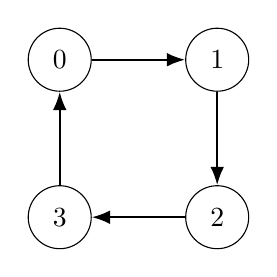
\begin{tikzpicture}[
    every node/.style={circle, draw, minimum size=0.8cm},
    edge/.style={-{Latex}, thick}
]
\node (0) at (0,0) {0};
\node (1) at (2,0) {1};
\node (2) at (2,-2) {2};
\node (3) at (0,-2) {3};

\draw[edge] (0) -- (1);
\draw[edge] (1) -- (2);
\draw[edge] (2) -- (3);
\draw[edge] (3) -- (0);
\end{tikzpicture}
\end{center}
\end{example}

\begin{definition}[Directed vs.\ undirected]
A graph is \textbf{undirected} if each edge is an unordered pair $\{u, v\}$. It is \textbf{directed} (or a \textbf{digraph}) if each edge is an ordered pair $(u, v)$, meaning the edge goes from $u$ to $v$.
\end{definition}

\begin{example}
An undirected edge $\{0, 1\}$ allows travel from $0$ to $1$ and from $1$ to $0$. A directed edge $(0, 1)$ allows travel only from $0$ to $1$.
\begin{center}
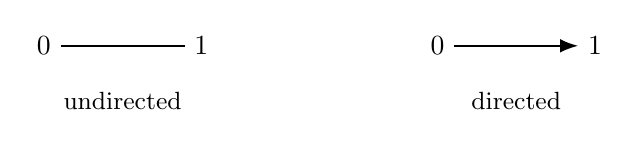
\begin{tikzpicture}
% Undirected (no arrow, no circle)
\node (u0) at (0,0) {0};
\node (u1) at (2,0) {1};
\draw[thick] (u0) -- (u1);
\node at (1,-0.7) {\small undirected};

% Directed (with arrow, no circle)
\node (d0) at (5,0) {0};
\node (d1) at (7,0) {1};
\draw[-{Latex}, thick] (d0) -- (d1);
\node at (6,-0.7) {\small directed};
\end{tikzpicture}
\end{center}
\end{example}

\begin{definition}[Weighted graph]
A \textbf{weighted graph} is a graph where each edge $(u, v)$ has a \textbf{weight} $w(u, v)$, typically a real number (positive, negative, or zero).
\end{definition}

\begin{example}
A weighted graph where the edge $(0, 1)$ has weight $2$, and $(1, 2)$ has weight $5$:
\begin{center}
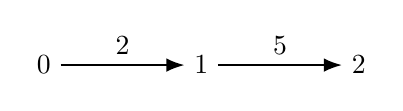
\begin{tikzpicture}
\node (0) at (0,0) {0};
\node (1) at (2,0) {1};
\node (2) at (4,0) {2};

\draw[-{Latex}, thick] (0) -- node[above] {2} (1);
\draw[-{Latex}, thick] (1) -- node[above] {5} (2);
\end{tikzpicture}
\end{center}
\end{example}

\begin{definition}[Degree]
In an undirected graph, the \textbf{degree} of a vertex $v$, denoted $\deg(v)$, is the number of edges incident to $v$. In a directed graph, we distinguish the \textbf{in-degree} (number of incoming edges) and the \textbf{out-degree} (number of outgoing edges).
\end{definition}

\begin{example}
In the directed graph below, we distinguish the \textbf{in-degree} (number of incoming edges) and the \textbf{out-degree} (number of outgoing edges):
\[
\begin{array}{c|cccc}
 & 0 & 1 & 2 & 3 \\
\hline
\text{in-degree} & 1 & 1 & 2 & 1 \\
\text{out-degree} & 2 & 2 & 0 & 1 \\
\end{array}
\]
\begin{center}
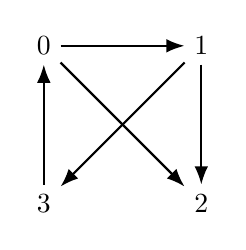
\begin{tikzpicture}
\node (0) at (0,0) {0};
\node (1) at (2,0) {1};
\node (2) at (2,-2) {2};
\node (3) at (0,-2) {3};

\draw[-{Latex}, thick] (0) -- (1);
\draw[-{Latex}, thick] (0) -- (2);
\draw[-{Latex}, thick] (1) -- (2);
\draw[-{Latex}, thick] (1) -- (3);
\draw[-{Latex}, thick] (3) -- (0);
\end{tikzpicture}
\end{center}
\end{example}

\begin{definition}[Path and cycle]
A \textbf{path} from $u$ to $v$ is a sequence of vertices $u = v_0, v_1, \ldots, v_k = v$ such that $(v_{i-1}, v_i) \in E$ for all $i$. The \textbf{length} of the path is the number of edges (or the sum of weights, if weighted).
A \textbf{cycle} is a path that starts and ends at the same vertex, with no repeated edges.
\end{definition}

\begin{example}
In the graph below, $0 \to 1 \to 2$ is a path of length 2. $0 \to 1 \to 2 \to 3 \to 0$ is a cycle of length 4.
\begin{center}
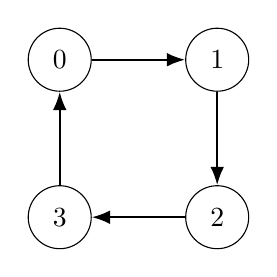
\begin{tikzpicture}[
    every node/.style={circle, draw, minimum size=0.8cm},
    edge/.style={-{Latex}, thick}
]
\node (0) at (0,0) {0};
\node (1) at (2,0) {1};
\node (2) at (2,-2) {2};
\node (3) at (0,-2) {3};

\draw[edge] (0) -- (1);
\draw[edge] (1) -- (2);
\draw[edge] (2) -- (3);
\draw[edge] (3) -- (0);
\end{tikzpicture}
\end{center}
\end{example}

\begin{definition}[Connected components]
An undirected graph is \textbf{connected} if there is a path between every pair of vertices. A \textbf{connected component} is a maximal connected subgraph.
\end{definition}

\begin{example}
The graph below has two connected components: $\{0, 1, 2\}$ and $\{3, 4\}$.
\begin{center}
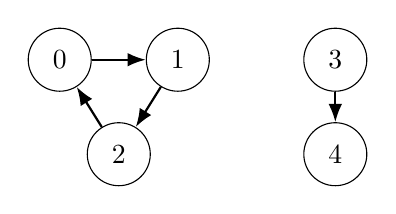
\begin{tikzpicture}[
    every node/.style={circle, draw, minimum size=0.8cm},
    edge/.style={-{Latex}, thick}
]
\node (0) at (0,0) {0};
\node (1) at (1.5,0) {1};
\node (2) at (0.75,-1.2) {2};
\node (3) at (3.5,0) {3};
\node (4) at (3.5,-1.2) {4};

\draw[edge] (0) -- (1);
\draw[edge] (1) -- (2);
\draw[edge] (2) -- (0);
\draw[edge] (3) -- (4);
\end{tikzpicture}
\end{center}
\end{example}

\begin{definition}[Strongly connected components]
A directed graph is \textbf{strongly connected} if there is a path from every vertex to every other vertex. A \textbf{strongly connected component} (SCC) is a maximal strongly connected subgraph.
\end{definition}

\begin{example}
In the directed graph below, $\{0, 1, 2\}$ is a strongly connected component (every vertex can reach every other), but $3$ is not (no path from $0$ to $3$, and no path from $3$ back to $0$).
\begin{center}
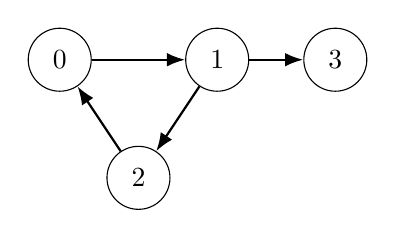
\begin{tikzpicture}[
    every node/.style={circle, draw, minimum size=0.8cm},
    edge/.style={-{Latex}, thick}
]
\node (0) at (0,0) {0};
\node (1) at (2,0) {1};
\node (2) at (1,-1.5) {2};
\node (3) at (3.5,0) {3};

\draw[edge] (0) -- (1);
\draw[edge] (1) -- (2);
\draw[edge] (2) -- (0);
\draw[edge] (1) -- (3);
\end{tikzpicture}
\end{center}
\end{example}

\begin{definition}[Tree]
A \textbf{tree} is a connected undirected graph with no cycles. Equivalently, a tree with $n$ vertices has exactly $n - 1$ edges.
\end{definition}

\begin{example}
A tree with 5 vertices and 4 edges:
\begin{center}
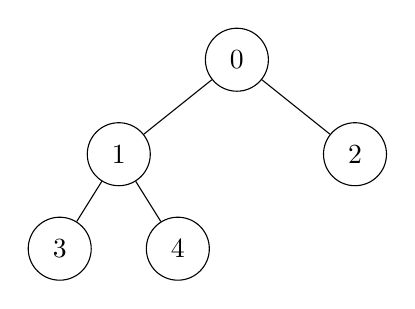
\begin{tikzpicture}[
    every node/.style={circle, draw, minimum size=0.8cm},
    edge/.style={-{Latex}, thick},
    level distance=1.2cm,
    level 1/.style={sibling distance=3cm},
    level 2/.style={sibling distance=1.5cm}
]
\node {0}
    child {node {1}
        child {node {3}}
        child {node {4}}
    }
    child {node {2}};
\end{tikzpicture}
\end{center}
\end{example}

\begin{definition}[DAG]
A \textbf{directed acyclic graph} (DAG) is a directed graph with no cycles.
\end{definition}

\begin{example}
A DAG representing dependencies (0 must be done before 1 and 2, 1 before 3):
\begin{center}
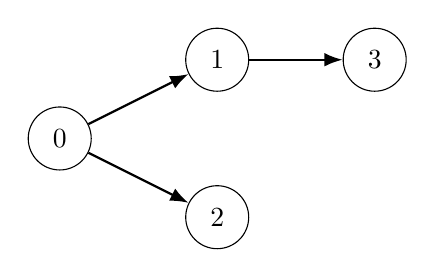
\begin{tikzpicture}[
    every node/.style={circle, draw, minimum size=0.8cm},
    edge/.style={-{Latex}, thick}
]
\node (0) at (0,0) {0};
\node (1) at (2,1) {1};
\node (2) at (2,-1) {2};
\node (3) at (4,1) {3};

\draw[edge] (0) -- (1);
\draw[edge] (0) -- (2);
\draw[edge] (1) -- (3);
\end{tikzpicture}
\end{center}
\end{example}

% ============================================================
% 2. REPRESENTATIONS
% ============================================================
\section{Representations}

A graph can be represented in two main ways.

\subsection{Adjacency Matrix}

A matrix $M$ of size $V \times V$, where:
\[
M[i][j] = \begin{cases}
w(i, j) & \text{if } (i, j) \in E, \\
0 \text{ or } \infty & \text{otherwise.}
\end{cases}
\]

\begin{center}
\begin{tabular}{lcc}
\toprule
Operation & Complexity \\
\midrule
Space & $O(V^2)$ \\
Edge test & $O(1)$ \\
Iterate neighbors & $O(V)$ \\
\bottomrule
\end{tabular}
\end{center}

\subsection{Adjacency List}

An array of lists, where $\text{adj}[u]$ contains all neighbors of $u$ (with weights, if weighted).

\begin{center}
\begin{tabular}{lcc}
\toprule
Operation & Complexity \\
\midrule
Space & $O(V + E)$ \\
Edge test & $O(\deg(u))$ \\
Iterate neighbors & $O(\deg(u))$ \\
\bottomrule
\end{tabular}
\end{center}

\begin{example}
For a graph with $V = 5$ and $E = 6$:
\begin{itemize}
    \item Adjacency matrix: $5 \times 5 = 25$ cells.
    \item Adjacency list: $5 + 2 \times 6 = 17$ entries (each undirected edge appears twice).
\end{itemize}
For sparse graphs ($E \ll V^2$), the list is more efficient.
\end{example}

\begin{example}[One graph, two representations]
Consider the following undirected, unweighted graph with $V = \{0, 1, 2, 3\}$ and edges $\{0,1\}, \{0,2\}, \{1,2\}, \{2,3\}$.

\begin{center}
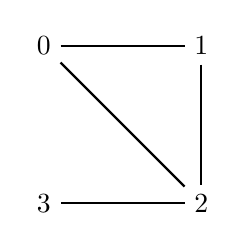
\begin{tikzpicture}
\node (0) at (0,0) {0};
\node (1) at (2,0) {1};
\node (2) at (2,-2) {2};
\node (3) at (0,-2) {3};

\draw[thick] (0) -- (1);
\draw[thick] (0) -- (2);
\draw[thick] (1) -- (2);
\draw[thick] (2) -- (3);
\end{tikzpicture}
\end{center}

\textbf{Adjacency matrix.} Since the graph has 4 vertices, the matrix is $4 \times 4$. Entry $M[i][j] = 1$ if there is an edge between $i$ and $j$, and $0$ otherwise:
\[
M =
\begin{pmatrix}
0 & 1 & 1 & 0 \\
1 & 0 & 1 & 0 \\
1 & 1 & 0 & 1 \\
0 & 0 & 1 & 0
\end{pmatrix}
\]
The matrix is symmetric (because the graph is undirected): $M[i][j] = M[j][i]$. It uses $4 \times 4 = 16$ cells, of which only 8 are non-zero (4 edges, each counted twice).

\textbf{Adjacency list.} The list is a \textbf{list of lists}: the $i$-th element is the list of neighbors of vertex $i$. For this graph:
\[
\mathrm{adj} = \bigl[\;[1, 2],\;\; [0, 2],\;\; [0, 1, 3],\;\; [2]\;\bigr]
\]
So $\mathrm{adj}[0] = [1, 2]$ means vertex 0 is connected to 1 and 2, $\mathrm{adj}[1] = [0, 2]$ means vertex 1 is connected to 0 and 2, and so on.

It uses $4 + 2 \times 4 = 12$ entries (4 vertices + 8 edge entries, since each undirected edge appears twice).

\textbf{Comparison.} The matrix uses $O(V^2)$ space and allows $O(1)$ edge tests, while the list uses $O(V + E)$ space and allows $O(\deg(u))$ edge tests. For sparse graphs ($E \ll V^2$), the list is more efficient; for dense graphs ($E \approx V^2$), the matrix may be competitive.
\end{example}

% ============================================================
% 3. BFS
% ============================================================
\section{Breadth-First Search (BFS)}

BFS explores the graph \textbf{level by level}, using a \textbf{queue}. It computes the shortest path in terms of \textbf{number of edges} from a source to all reachable vertices.

\subsection{Algorithm}

\begin{lstlisting}
from collections import deque

def bfs(graph, start):
    visited = {start}
    queue = deque([start])
    dist = {start: 0}
    while queue:
        u = queue.popleft()
        for v in graph[u]:
            if v not in visited:
                visited.add(v)
                dist[v] = dist[u] + 1
                queue.append(v)
    return dist
\end{lstlisting}

\subsection{Example}

\begin{center}
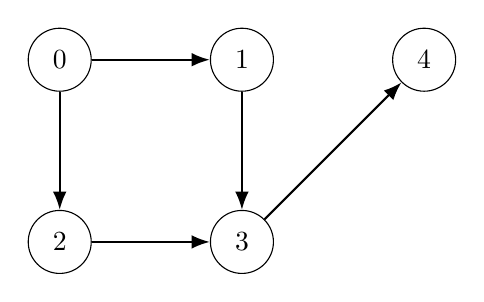
\begin{tikzpicture}[
    node distance=1.5cm,
    every node/.style={circle, draw, minimum size=0.8cm},
    edge/.style={-{Latex}, thick}
]
\node (0) {0};
\node (1) [right=of 0] {1};
\node (2) [below=of 0] {2};
\node (3) [below=of 1] {3};
\node (4) [right=of 1] {4};

\draw[edge] (0) -- (1);
\draw[edge] (0) -- (2);
\draw[edge] (1) -- (3);
\draw[edge] (2) -- (3);
\draw[edge] (3) -- (4);
\end{tikzpicture}
\end{center}

BFS from 0: order of visits is $0, 1, 2, 3, 4$. Distances: $\{0: 0, 1: 1, 2: 1, 3: 2, 4: 3\}$.

\subsection{Complexity}

\begin{center}
\begin{tabular}{lcc}
\toprule
Resource & Adjacency list & Adjacency matrix \\
\midrule
Time & $O(V + E)$ & $O(V^2)$ \\
Space & $O(V)$ & $O(V)$ \\
\bottomrule
\end{tabular}
\end{center}

\subsection{Properties}

\begin{itemize}
    \item BFS visits vertices in increasing order of distance from the source.
    \item It is \textbf{optimal} for unweighted shortest paths.
    \item It does \textbf{not} work for weighted graphs (use Dijkstra instead).
\end{itemize}

% ============================================================
% 4. DFS
% ============================================================
\section{Depth-First Search (DFS)}

DFS explores as deep as possible before backtracking, using a \textbf{stack} (or recursion).

\subsection{Algorithm}

\begin{lstlisting}
def dfs(graph, u, visited=None):
    if visited is None:
        visited = set()
    visited.add(u)
    for v in graph[u]:
        if v not in visited:
            dfs(graph, v, visited)
    return visited
\end{lstlisting}

\subsection{Example}

Using the same graph as BFS, DFS from 0 visits: $0, 1, 3, 2, 4$ (one possible order, depending on the order of neighbors).

\subsection{Complexity}

\begin{center}
\begin{tabular}{lcc}
\toprule
Resource & Adjacency list & Adjacency matrix \\
\midrule
Time & $O(V + E)$ & $O(V^2)$ \\
Space & $O(V)$ & $O(V)$ \\
\bottomrule
\end{tabular}
\end{center}

\subsection{Applications}

\begin{itemize}
    \item Cycle detection (see Section~5).
    \item Topological sorting (see Section~5).
    \item Connected components.
    \item Strongly connected components.
\end{itemize}

% ============================================================
% 5. CYCLE DETECTION AND TOPOLOGICAL SORT
% ============================================================
\section{Cycle Detection and Topological Sort}

\subsection{Cycle Detection in an Undirected Graph}

In an undirected graph, a DFS with the parent of each vertex can detect cycles: if we encounter a visited vertex that is not the parent, there is a cycle.

\begin{lstlisting}
def has_cycle_undirected(graph):
    visited = set()

    def dfs(u, parent):
        visited.add(u)
        for v in graph[u]:
            if v not in visited:
                if dfs(v, u):
                    return True
            elif v != parent:
                return True
        return False

    for u in graph:
        if u not in visited:
            if dfs(u, None):
                return True
    return False
\end{lstlisting}

\textbf{Complexity:} $O(V + E)$.

\subsection{Cycle Detection in a Directed Graph}

In a directed graph, we use \textbf{three colors}:
\begin{itemize}
    \item \textbf{White}: not visited.
    \item \textbf{Gray}: in progress (on the recursion stack).
    \item \textbf{Black}: finished.
\end{itemize}

If we encounter a \textbf{gray} vertex, there is a cycle (back edge).

\begin{lstlisting}
def has_cycle_directed(graph):
    WHITE, GRAY, BLACK = 0, 1, 2
    color = {u: WHITE for u in graph}

    def dfs(u):
        color[u] = GRAY
        for v in graph[u]:
            if color[v] == GRAY:
                return True
            if color[v] == WHITE and dfs(v):
                return True
        color[u] = BLACK
        return False

    for u in graph:
        if color[u] == WHITE:
            if dfs(u):
                return True
    return False
\end{lstlisting}

\textbf{Complexity:} $O(V + E)$.

\subsection{Topological Sort (DAG)}

A \textbf{topological sort} of a DAG is a linear ordering of vertices such that for every edge $(u, v)$, $u$ appears before $v$. It exists if and only if the graph is a DAG.

\begin{lstlisting}
def topological_sort(graph):
    visited = set()
    order = []

    def dfs(u):
        visited.add(u)
        for v in graph[u]:
            if v not in visited:
                dfs(v)
        order.append(u)

    for u in graph:
        if u not in visited:
            dfs(u)
    return order[::-1]   # reverse post-order
\end{lstlisting}

\textbf{Complexity:} $O(V + E)$.

% ============================================================
% 6. CONNECTED COMPONENTS
% ============================================================
\section{Connected Components}

\subsection{Undirected Graphs}

A \textbf{connected component} is a maximal set of vertices where every pair is connected by a path. We can find them with BFS or DFS:

\begin{lstlisting}
def connected_components(graph):
    visited = set()
    components = []

    def dfs(u, component):
        visited.add(u)
        component.append(u)
        for v in graph[u]:
            if v not in visited:
                dfs(v, component)

    for u in graph:
        if u not in visited:
            component = []
            dfs(u, component)
            components.append(component)
    return components
\end{lstlisting}

\textbf{Complexity:} $O(V + E)$.

\subsection{Strongly Connected Components (Directed Graphs)}

A \textbf{strongly connected component} (SCC) is a maximal set of vertices where every vertex can reach every other. The two classic algorithms are:
\begin{itemize}
    \item \textbf{Kosaraju's algorithm}: two DFS passes (one on the graph, one on the transpose).
    \item \textbf{Tarjan's algorithm}: one DFS pass with a stack and low-link values.
\end{itemize}

Both run in $O(V + E)$.

% ============================================================
% 7. WEIGHTED GRAPHS
% ============================================================
\section{Weighted Graphs}

In a \textbf{weighted graph}, each edge $(u, v)$ has a weight $w(u, v)$. The \textbf{shortest path} between two vertices is the path with minimum total weight.

\subsection{Dijkstra's Algorithm}

Dijkstra finds the shortest paths from a source to all vertices, assuming \textbf{all edge weights are non-negative}.

\subsubsection{Algorithm}

\begin{lstlisting}
import heapq

def dijkstra(graph, source):
    dist = {u: float('inf') for u in graph}
    dist[source] = 0
    pq = [(0, source)]
    while pq:
        d, u = heapq.heappop(pq)
        if d > dist[u]:
            continue
        for v, w in graph[u]:
            nd = d + w
            if nd < dist[v]:
                dist[v] = nd
                heapq.heappush(pq, (nd, v))
    return dist
\end{lstlisting}

\textbf{Complexity:} $O((V + E) \log V)$ with a binary heap.

\textbf{Limitation:} Dijkstra \textbf{fails with negative edge weights}. A negative edge could create a shorter path to an already-finalized vertex.

\subsubsection{Example}

\begin{center}
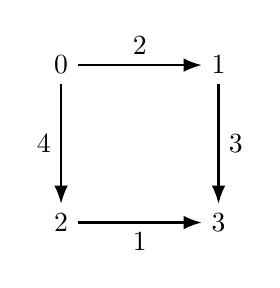
\begin{tikzpicture}
\node (0) at (0,0) {0};
\node (1) at (2,0) {1};
\node (2) at (0,-2) {2};
\node (3) at (2,-2) {3};

\draw[-{Latex}, thick] (0) -- node[above] {2} (1);
\draw[-{Latex}, thick] (0) -- node[left] {4} (2);
\draw[-{Latex}, thick] (1) -- node[right] {3} (3);
\draw[-{Latex}, thick] (2) -- node[below] {1} (3);
\end{tikzpicture}
\end{center}

Dijkstra from 0: $\{0: 0, 1: 2, 2: 4, 3: 5\}$ (path $0 \to 2 \to 3$ has weight $4 + 1 = 5$, same as $0 \to 1 \to 3$ with $2 + 3 = 5$).

\subsection{Dijkstra's Algorithm Without a Heap}

The heap version is optimal for sparse graphs, but for \textbf{dense graphs} ($E \approx V^2$), a simpler version using an array is actually faster.

\subsubsection{Idea}

Instead of a priority queue, maintain:
\begin{itemize}
    \item \code{dist[v]}: the current best-known distance from the source to \code{v}.
    \item \code{visited[v]}: whether \code{v} has been finalized (its distance is final).
\end{itemize}

At each step:
\begin{enumerate}
    \item Find the \textbf{unvisited vertex with the smallest \code{dist}} (linear scan over all vertices).
    \item Mark it as visited.
    \item \textbf{Relax} its outgoing edges: for each neighbor \code{v} with weight \code{w}, if \code{dist[u] + w < dist[v]}, update \code{dist[v]}.
\end{enumerate}

Repeat until all vertices are visited (or the smallest distance is infinity, meaning the remaining vertices are unreachable).

\subsubsection{Algorithm}

\begin{lstlisting}
def dijkstra_array(graph, source):
    n = len(graph)
    dist = [float('inf')] * n
    visited = [False] * n
    dist[source] = 0

    for _ in range(n):
        # Step 1: find the unvisited vertex with the smallest distance
        u = -1
        best = float('inf')
        for v in range(n):
            if not visited[v] and dist[v] < best:
                best = dist[v]
                u = v

        # If no reachable vertex remains, stop
        if u == -1:
            break

        # Step 2: mark u as visited
        visited[u] = True

        # Step 3: relax the outgoing edges of u
        for v, w in graph[u]:
            if dist[u] + w < dist[v]:
                dist[v] = dist[u] + w

    return dist
\end{lstlisting}

\textbf{Input:} an adjacency list where \code{graph[u]} is a list of \code{(v, w)} pairs. Vertices are numbered \code{0} to \code{n-1}.

\textbf{Output:} a list \code{dist} where \code{dist[v]} is the shortest distance from \code{source} to \code{v} (or \code{inf} if unreachable).

\subsubsection{Example}

Same graph as above:

\begin{center}
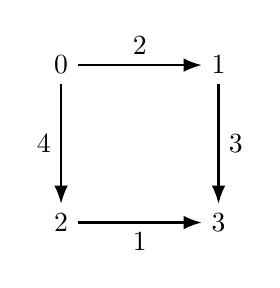
\begin{tikzpicture}
\node (0) at (0,0) {0};
\node (1) at (2,0) {1};
\node (2) at (0,-2) {2};
\node (3) at (2,-2) {3};

\draw[-{Latex}, thick] (0) -- node[above] {2} (1);
\draw[-{Latex}, thick] (0) -- node[left] {4} (2);
\draw[-{Latex}, thick] (1) -- node[right] {3} (3);
\draw[-{Latex}, thick] (2) -- node[below] {1} (3);
\end{tikzpicture}
\end{center}

Trace from source 0:

\textbf{Initial:}
\[
\text{dist} = [0, \infty, \infty, \infty], \quad \text{visited} = [F, F, F, F]
\]

\textbf{Step 1:} smallest unvisited is 0 (dist = 0). Mark visited.
Relax edges of 0:
\begin{itemize}
    \item $0 \to 1$ (weight 2): \code{dist[1] = 0 + 2 = 2}.
    \item $0 \to 2$ (weight 4): \code{dist[2] = 0 + 4 = 4}.
\end{itemize}
\[
\text{dist} = [0, 2, 4, \infty], \quad \text{visited} = [T, F, F, F]
\]

\textbf{Step 2:} smallest unvisited is 1 (dist = 2). Mark visited.
Relax edges of 1:
\begin{itemize}
    \item $1 \to 3$ (weight 3): \code{dist[3] = 2 + 3 = 5}.
\end{itemize}
\[
\text{dist} = [0, 2, 4, 5], \quad \text{visited} = [T, T, F, F]
\]

\textbf{Step 3:} smallest unvisited is 2 (dist = 4). Mark visited.
Relax edges of 2:
\begin{itemize}
    \item $2 \to 3$ (weight 1): $4 + 1 = 5$, not better than 5. No update.
\end{itemize}
\[
\text{dist} = [0, 2, 4, 5], \quad \text{visited} = [T, T, T, F]
\]

\textbf{Step 4:} smallest unvisited is 3 (dist = 5). Mark visited.
No outgoing edges.
\[
\text{dist} = [0, 2, 4, 5], \quad \text{visited} = [T, T, T, T]
\]

\textbf{Result:} $[0, 2, 4, 5]$. The shortest distances from 0 are: to 0 = 0, to 1 = 2, to 2 = 4, to 3 = 5.

\subsubsection{Complexity}

\begin{center}
\begin{tabular}{lcc}
\toprule
Resource & Array version & Heap version \\
\midrule
Time & $O(V^2)$ & $O((V + E) \log V)$ \\
Space & $O(V)$ & $O(V + E)$ \\
Best for & Dense graphs & Sparse graphs \\
\bottomrule
\end{tabular}
\end{center}

\textbf{Why $O(V^2)$:} the outer loop runs $V$ times, and each iteration does a linear scan of $V$ vertices to find the minimum. The total relaxation cost is $O(E)$, which is dominated by $O(V^2)$ for dense graphs.

\subsubsection{Correctness}

\textbf{Invariant:} when a vertex $u$ is marked as visited, \code{dist[u]} is the true shortest distance from the source.

\textbf{Proof (by induction on the number of visited vertices):}

\begin{itemize}
    \item \textbf{Base case:} the source is visited first, with \code{dist[source] = 0}. Correct.
    \item \textbf{Inductive step:} suppose all previously visited vertices have correct distances. Let $u$ be the unvisited vertex with the smallest \code{dist[u]}. We claim \code{dist[u]} is the true shortest distance.
    \begin{itemize}
        \item Suppose there is a shorter path from the source to $u$. This path must go through some unvisited vertex $x$ (since all visited vertices have correct distances, and any path through them would already be reflected in \code{dist[u]}).
        \item But $x$ is unvisited, and \code{dist[x]} $\geq$ \code{dist[u]} (since $u$ is the minimum). So the path through $x$ has length at least \code{dist[u]}, contradiction.
        \item Therefore, \code{dist[u]} is correct.
    \end{itemize}
\end{itemize}

Since all edge weights are non-negative, the greedy choice is safe. $\qed$

\subsection{Floyd-Warshall Algorithm}

Floyd-Warshall computes the shortest paths between \textbf{all pairs} of vertices, using dynamic programming.

\subsubsection{Algorithm}

\begin{lstlisting}
def floyd_warshall(adj_matrix):
    n = len(adj_matrix)
    dist = [row[:] for row in adj_matrix]
    for k in range(n):
        for i in range(n):
            for j in range(n):
                if dist[i][k] + dist[k][j] < dist[i][j]:
                    dist[i][j] = dist[i][k] + dist[k][j]
    return dist
\end{lstlisting}

\textbf{Input:} an adjacency matrix where \code{adj_matrix[i][j]} is the weight of edge $i \to j$, or \code{float('inf')} if absent, and 0 for $i = j$.

\textbf{Output:} a matrix \code{dist} where \code{dist[i][j]} is the shortest distance from $i$ to $j$.

\subsubsection{Complexity}

\begin{center}
\begin{tabular}{lc}
\toprule
Resource & Complexity \\
\midrule
Time & $O(V^3)$ \\
Space & $O(V^2)$ \\
\bottomrule
\end{tabular}
\end{center}

\textbf{Why $O(V^3)$:} three nested loops, each running $V$ times. The inner loop body is $O(1)$.

\subsubsection{Properties}

\begin{itemize}
    \item Handles \textbf{negative edge weights} (but not negative cycles).
    \item Simple to implement (three nested loops).
    \item Best for \textbf{dense graphs} or when all-pairs distances are needed.
\end{itemize}

\textbf{Negative cycle detection:} after the algorithm, if $\text{dist}[i][i] < 0$ for some $i$, there is a negative cycle through $i$.

\subsubsection{Example}

Graph with 4 vertices:

\begin{center}
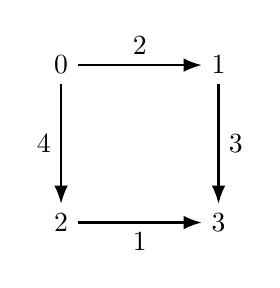
\begin{tikzpicture}
\node (0) at (0,0) {0};
\node (1) at (2,0) {1};
\node (2) at (0,-2) {2};
\node (3) at (2,-2) {3};

\draw[-{Latex}, thick] (0) -- node[above] {2} (1);
\draw[-{Latex}, thick] (0) -- node[left] {4} (2);
\draw[-{Latex}, thick] (1) -- node[right] {3} (3);
\draw[-{Latex}, thick] (2) -- node[below] {1} (3);
\end{tikzpicture}
\end{center}

Adjacency matrix:
\[
\text{adj} =
\begin{pmatrix}
0 & 2 & 4 & \infty \\
\infty & 0 & \infty & 3 \\
\infty & \infty & 0 & 1 \\
\infty & \infty & \infty & 0
\end{pmatrix}
\]

After Floyd-Warshall:
\[
\text{dist} =
\begin{pmatrix}
0 & 2 & 4 & 5 \\
\infty & 0 & \infty & 3 \\
\infty & \infty & 0 & 1 \\
\infty & \infty & \infty & 0
\end{pmatrix}
\]

The shortest distances from 0 are: to 0 = 0, to 1 = 2, to 2 = 4, to 3 = 5 (via $0 \to 2 \to 3$).

\subsection{Comparison}

\begin{center}
\renewcommand{\arraystretch}{1.2}
\small
\begin{tabular}{lcccc}
\toprule
Algorithm & Problem & Negative weights? & Time & Space \\
\midrule
Dijkstra (heap) & Single-source & No & $O((V + E) \log V)$ & $O(V + E)$ \\
Dijkstra (array) & Single-source & No & $O(V^2)$ & $O(V)$ \\
Floyd-Warshall & All-pairs & Yes (no neg.\ cycles) & $O(V^3)$ & $O(V^2)$ \\
\bottomrule
\end{tabular}
\end{center}

\textbf{When to use which:}
\begin{itemize}
    \item \textbf{Dijkstra (heap)}: single-source shortest paths, sparse graphs, non-negative weights.
    \item \textbf{Dijkstra (array)}: single-source shortest paths, dense graphs, non-negative weights.
    \item \textbf{Floyd-Warshall}: all-pairs shortest paths, dense graphs, negative weights allowed.
\end{itemize}

% ============================================================
% 8. COMPARISON
% ============================================================
\section{Comparison of Algorithms}

\begin{center}
\renewcommand{\arraystretch}{1.3}
\small
\begin{tabular}{>{\raggedright\arraybackslash}p{3cm} >{\raggedright\arraybackslash}p{3cm} >{\raggedright\arraybackslash}p{3cm} >{\raggedright\arraybackslash}p{3cm}}
\toprule
Algorithm & Problem & Negative weights? & Complexity \\
\midrule
BFS & Single-source, unweighted & --- & $O(V + E)$ \\
DFS & Traversal, cycles & --- & $O(V + E)$ \\
Dijkstra & Single-source, non-negative & No & $O((V + E) \log V)$ \\
Floyd-Warshall & All-pairs, any weights (no neg.\ cycles) & Yes & $O(V^3)$ \\
\bottomrule
\end{tabular}
\end{center}

\textbf{When to use which:}
\begin{itemize}
    \item \textbf{BFS}: unweighted shortest paths, connected components.
    \item \textbf{DFS}: cycle detection, topological sort, SCC.
    \item \textbf{Dijkstra}: single-source shortest paths with non-negative weights.
    \item \textbf{Floyd-Warshall}: all-pairs shortest paths, dense graphs, negative weights.
\end{itemize}

\end{document}